\chapter{Analyse}
\label{chap:analyse}

Ce chapitre présente l'analyse des risques liés à l'utilisation de la station de gravure laser intelligente, ainsi que la prise en main du bras robot Ufactory Xarm6 et du logiciel AICA Studio. Il s'agit d'une étape de découverte et d'apprentissage des outils et des technologies utilisées. Cela permet également de prouver le faisabilité du projet.

\section{Analyse des risques}
L'utilisation d'une station de gravure laser intelligente avec un bras robotisé en environnement public comporte plusieurs risques qu'il convient d'identifier, d'évaluer et de maîtriser. L'analyse suivante s'appuie sur le contexte du projet, les éléments matériels et logiciels utilisés, ainsi que les objectifs de sécurité et de fiabilité.

\subsection{Risques identifiés}
\begin{itemize}
    \item \textbf{Risque laser} : Le laser utilisé pour la gravure présente un danger pour la vue et la peau en cas d'exposition accidentelle. Un mauvais contrôle logiciel ou une défaillance matérielle pourrait entraîner l'activation du laser hors de la zone prévue.
    \item \textbf{Risque robotique} : Le bras robot Ufactory Xarm6, bien que collaboratif, reste potentiellement dangereux. Il peut provoquer des blessures par collision ou pincement si un utilisateur s'approche trop près pendant le fonctionnement. Une sous section est dédiée à l'analyse de risques concernant le robot.
    \item \textbf{Risque électrique} : La station comporte plusieurs alimentations électriques (robot, laser, écran tactile) pouvant présenter un danger en cas de défaut d'isolation ou de manipulation inappropriée. Notamment au niveau des alimentations 230V des différents éléments.
    \item \textbf{Risque logiciel et synchronisation} : Une erreur dans la synchronisation entre le robot et le laser pourrait activer le laser au mauvais moment ou déplacer le robot de façon imprévue.
    \item \textbf{Risque de mauvaise détection} : Une défaillance de la caméra ou une erreur dans le traitement des données pourrait entraîner une mauvaise localisation de la pièce à graver, provoquant des collisions ou des gravures hors zone.
    \item \textbf{Risque d'utilisation publique} : En contexte de démonstration, le public peut adopter des comportements imprévisibles (toucher, interférer, etc.), augmentant les risques d'accident.
\end{itemize}

\subsection{Risque robotique}

\rowcolors{2}{white}{gray!10}
\begin{table}[H]
    \centering
    \renewcommand{\arraystretch}{1.4}
    \begin{tabular}{|p{3.5cm}|>{\centering\arraybackslash}m{2.2cm}|>{\centering\arraybackslash}m{2.2cm}|>{\centering\arraybackslash}m{2.2cm}|p{3.5cm}|}
        \hline
        \textbf{Risque} & \textbf{Sévérité} & \textbf{Fréquence} & \textbf{Importance} & \textbf{Description} \\
        \hline
        Collision avec un utilisateur & \cellcolor{orange!60}Moyenne & \cellcolor{yellow!60}Faible & \cellcolor{orange!60}Moyenne & Blessure possible en cas de contact entre le bras robot et une personne. \\
        \hline
        Pincement lors du mouvement & \cellcolor{green!60}Très Faible & \cellcolor{yellow!60}Faible & \cellcolor{yellow!60}Faible & Risque de pincement des doigts ou de la main lors des mouvements du robot, notamment avec la pince. \\
        \hline
        Mauvaise préhension de la pièce & \cellcolor{yellow!60}Faible & \cellcolor{red!60}Élevée & \cellcolor{orange!60}Moyenne & Le robot peut mal saisir la pièce, entraînant des erreurs de positionnement et des comportements imprévus. \\
        \hline
        Mouvement imprévu suite à une erreur logicielle & \cellcolor{yellow!60}Faible & \cellcolor{green!60}Très faible & \cellcolor{yellow!60}Faible & Un bug logiciel peut entraîner un déplacement non anticipé du robot. \\
        \hline
        Défaillance du système de sécurité & \cellcolor{red!60}Élevée & \cellcolor{green!60}Très faible & \cellcolor{orange!60}Moyenne & Si les dispositifs de sécurité ne fonctionnent pas, le robot peut devenir dangereux. \\
        \hline
    \end{tabular}
    \caption{Tableau d'analyse des risques robotiques pour le bras Ufactory Xarm6 dans le cadre de l'utilisation de la station de gravure laser intelligente.}
    \label{tab:risques_robotique}
\end{table}

Cette analyse permet de mettre en place des mesures de sécurité pour la station, en anticipant les principaux scénarios à risque.

\subsection{Mesures de prévention et de maîtrise}
\begin{itemize}
    \item Mise en place de protections physiques (capot, barrières) autour de la zone de gravure. (à mettre en place)
    \item Activation du laser uniquement lorsque le robot est en position sécurisée et la zone libre.
    \item Surveillance logicielle de la synchronisation robot/laser et gestion des erreurs critiques.
    \item Validation logicielle de la détection de pièce et limitation des mouvements du robot en cas d'incertitude.
    \item Présence d'un opérateur formé lors des démonstrations publiques.
    \item Ajout d'une vérification de prise de pièce via une caméra.
\end{itemize}

Ces mesures permettent de réduire significativement les risques identifiés, en garantissant un fonctionnement sécurisé et fiable de la station de gravure laser intelligente.

L'ajout de ces sécurités a été fait au fur et à mesure du développement du projet. L'ajout de la verification de la prise de pièce via une caméra a été implémenté en dernier suite à une réflexion sur les potentielles amélioration et fiabilisations du système. En effet, la vérification de la prise de pièce permet de s'assurer que le robot a bien saisi la pièce avant de se déplacer vers la zone de gravure, réduisant ainsi les risques que la graveuse laser active le laser dans le vide.


\section{Prise en main du bras robot}
La prise en main du bras robot Ufactory Xarm6 a été une des premières étapes du projet. Le but était de se familiariser avec les commandes et de comprendre les limites physiques et logicielles du robot.

\subsection{Mise en marche du robot et connexion}
Avec le manuel utilisateur fourni par Ufactory \cite{UserManual}, il a été possible de comprendre et prendre en main le robot. La première étape après la mise sous tension à été la connexion ethernet entre le contrôleur et le logiciel UFACTORY-Studio. La procédure est très simple et ne demande pas de configuration particulière.

\subsection{UFACTORY-Studio}
Le logiciel UFACTORY-Studio est utile pour configurer la position initiale du robot, les limites de mouvements, la force maximale de chaque articulation et les limites de distances à ne pas dépasser.

En plus de cela, le logiciel offre un contrôle complet sur les entrées/sorties (appelées à partir de maintenant \gls{io}), les axes, la vitesse de déplacement et l'ouverture/fermeture de la pince. Il est également possible de créer des programmes de mouvement en utilisant le langage  de programation Python ou un langage visuel propriétaire basé sur le Python. Le langage visuel reste très basique et ne permet pas de créer des programmes complexes qui sortent du cadre de la cinématique du robot.

\subsection{Python SDK}
Pour s'affranchir des limitations du logiciel UFACTORY-Studio, il est possible d'utiliser le \gls{sdk} Python \cite{PythonSDK} fourni par Ufactory. Ce SDK permet de contrôler le robot de manière plus avancée et de créer des programmes plus complexes. Le langage de base de contrôle du robot étant le Python, il est possible d'utiliser n'importe quel IDE Python pour développer des programmes. La documentation du SDK étant très complète avec de nombreux exemples, la compréhension et la prise en main du SDK se sont faites rapidement. De plus, les contrôles de cinématique sont plus "bas niveau" ce qui offre plus de flexibilité notamment au niveau de l'accéleration, du \gls{jerk} et des opérations sur les positions.

\subsection{Entrées/sorties}
Le contrôleur du bras robot offre plusieurs types d'IO:

\definecolor{SafetyColor}{HTML}{FFDDC1}
\definecolor{PowerColor}{HTML}{C1E1FF}
\definecolor{ConfigInputColor}{HTML}{D4FFC1}
\definecolor{DigitalInputColor}{HTML}{FFD1DC}
\definecolor{ConfigOutputColor}{HTML}{E1C1FF}
\definecolor{DigitalOutputColor}{HTML}{C1FFE1}
\definecolor{RS485Color}{HTML}{FFC1E1}
\definecolor{AnalogColor}{HTML}{E1FFC1}

\begin{tcolorbox}[colframe=black, colback=SafetyColor, title=Safety]
    \textbf{Connexions :} GND | EI0 | GND | EI1 | GND | SI0 | GND | SI1
\end{tcolorbox}

\begin{tcolorbox}[colframe=black, colback=PowerColor, title=Power]
    \textbf{Connexions :} PWR | 24V-IN | GND | RI0 | NC | GND | ON | OFF
\end{tcolorbox}

\begin{tcolorbox}[colframe=black, colback=ConfigInputColor, title=Configurable Inputs]
    \textbf{Connexions :} GND | CI0 | CI1 | CI2 | CI3 | GND | CI4 | CI5 |CI6 | CI7
\end{tcolorbox}

\begin{tcolorbox}[colframe=black, colback=DigitalInputColor, title=Digital Inputs]
    \textbf{Connexions :} GND |  DI0 | DI1 | DI2 | DI3 | GND | DI4 | DI5 | DI6 | DI7
\end{tcolorbox}

\begin{tcolorbox}[colframe=black, colback=ConfigOutputColor, title=Configurable Outputs]
    \textbf{Connexions :} 24V | CO0 | CO1 | CO2 | CO3 | 24V | CO4 | CO5 | CO6 | CO7
\end{tcolorbox}

\begin{tcolorbox}[colframe=black, colback=DigitalOutputColor, title=Digital Outputs]
    \textbf{Connexions :} 24V | DO0 | DO1 | DO2 | DO3 | 24V | DO4 | DO5 | DO6 | DO7
\end{tcolorbox}

\begin{tcolorbox}[colframe=black, colback=RS485Color, title=RS485]
    \textbf{Connexions :} 24V | 24V | M\_A | M\_B | GND | L\_A | L\_B | GND
\end{tcolorbox}

\begin{tcolorbox}[colframe=black, colback=AnalogColor, title=Analog]
    \textbf{Connexions :} GND | AI0 | GND | AI1 | GND | AO0 | GND | AO1
\end{tcolorbox}

Ces IO premettent la communication avec des éléments externes.

\section{AICA Studio}
AICA Studio est un logiciel qui simplifie l'intégration et la programmation de robots industriels via des blocs de fonctions prédéfinis. Il est compatible avec le bras robot Ufactory Xarm6 et permet de créer des programmes de manière visuelle, sans nécessiter de compétences avancées en programmation. Le logiciel s'appuie sur \gls{ros2}, qui gère les aspects bas-niveau du contrôle et de la communication, tandis que AICA, en tant que couche supérieure, propose une interface simplifiée pour la gestion des tâches complexes, telles que la planification de trajectoires ou l'intégration d'opérations avancées comme la détection de collisions ou le contrôle du robot avec l'interface \gls{rviz}.

\subsection{Installation de AICA Studio}
L'installation de AICA Studio est, contrairement à UFACTORY-Studio, un peu plus complexe. Il est nécessaire d'utiliser un système d'exploitation Linux ou Posix. Le guide d'installation \cite{AICADocs} est complet et facile à suivre. Cependant, il est tout de même nécessaire d'avoir quelques connaissance de base en ligne de commandes et en gestion de systèmes Linux. L'avantage de cette installation est qu'elle permet de créer un environnement complet en incluant dans un \gls{conteneur} \gls{docker} tous les outils nécessaire au bon fonctionnement de l'application.

\subsection{Démarrage de AICA Studio}
Le démarrage de AICA Studio suit la procédure strandart des applications Linux. Lorsque l'application est lancée pour la première foi, une fenêtre de configuration s'ouvre pour permettre d'entrer la clef de licence. Par la suite, l'application se lance et affiche une page de réglages pour choisir la version, les packages à installer et les volumes partagés pour l'utilisation de fichiers.

\begin{figure}[H]
    \centering
    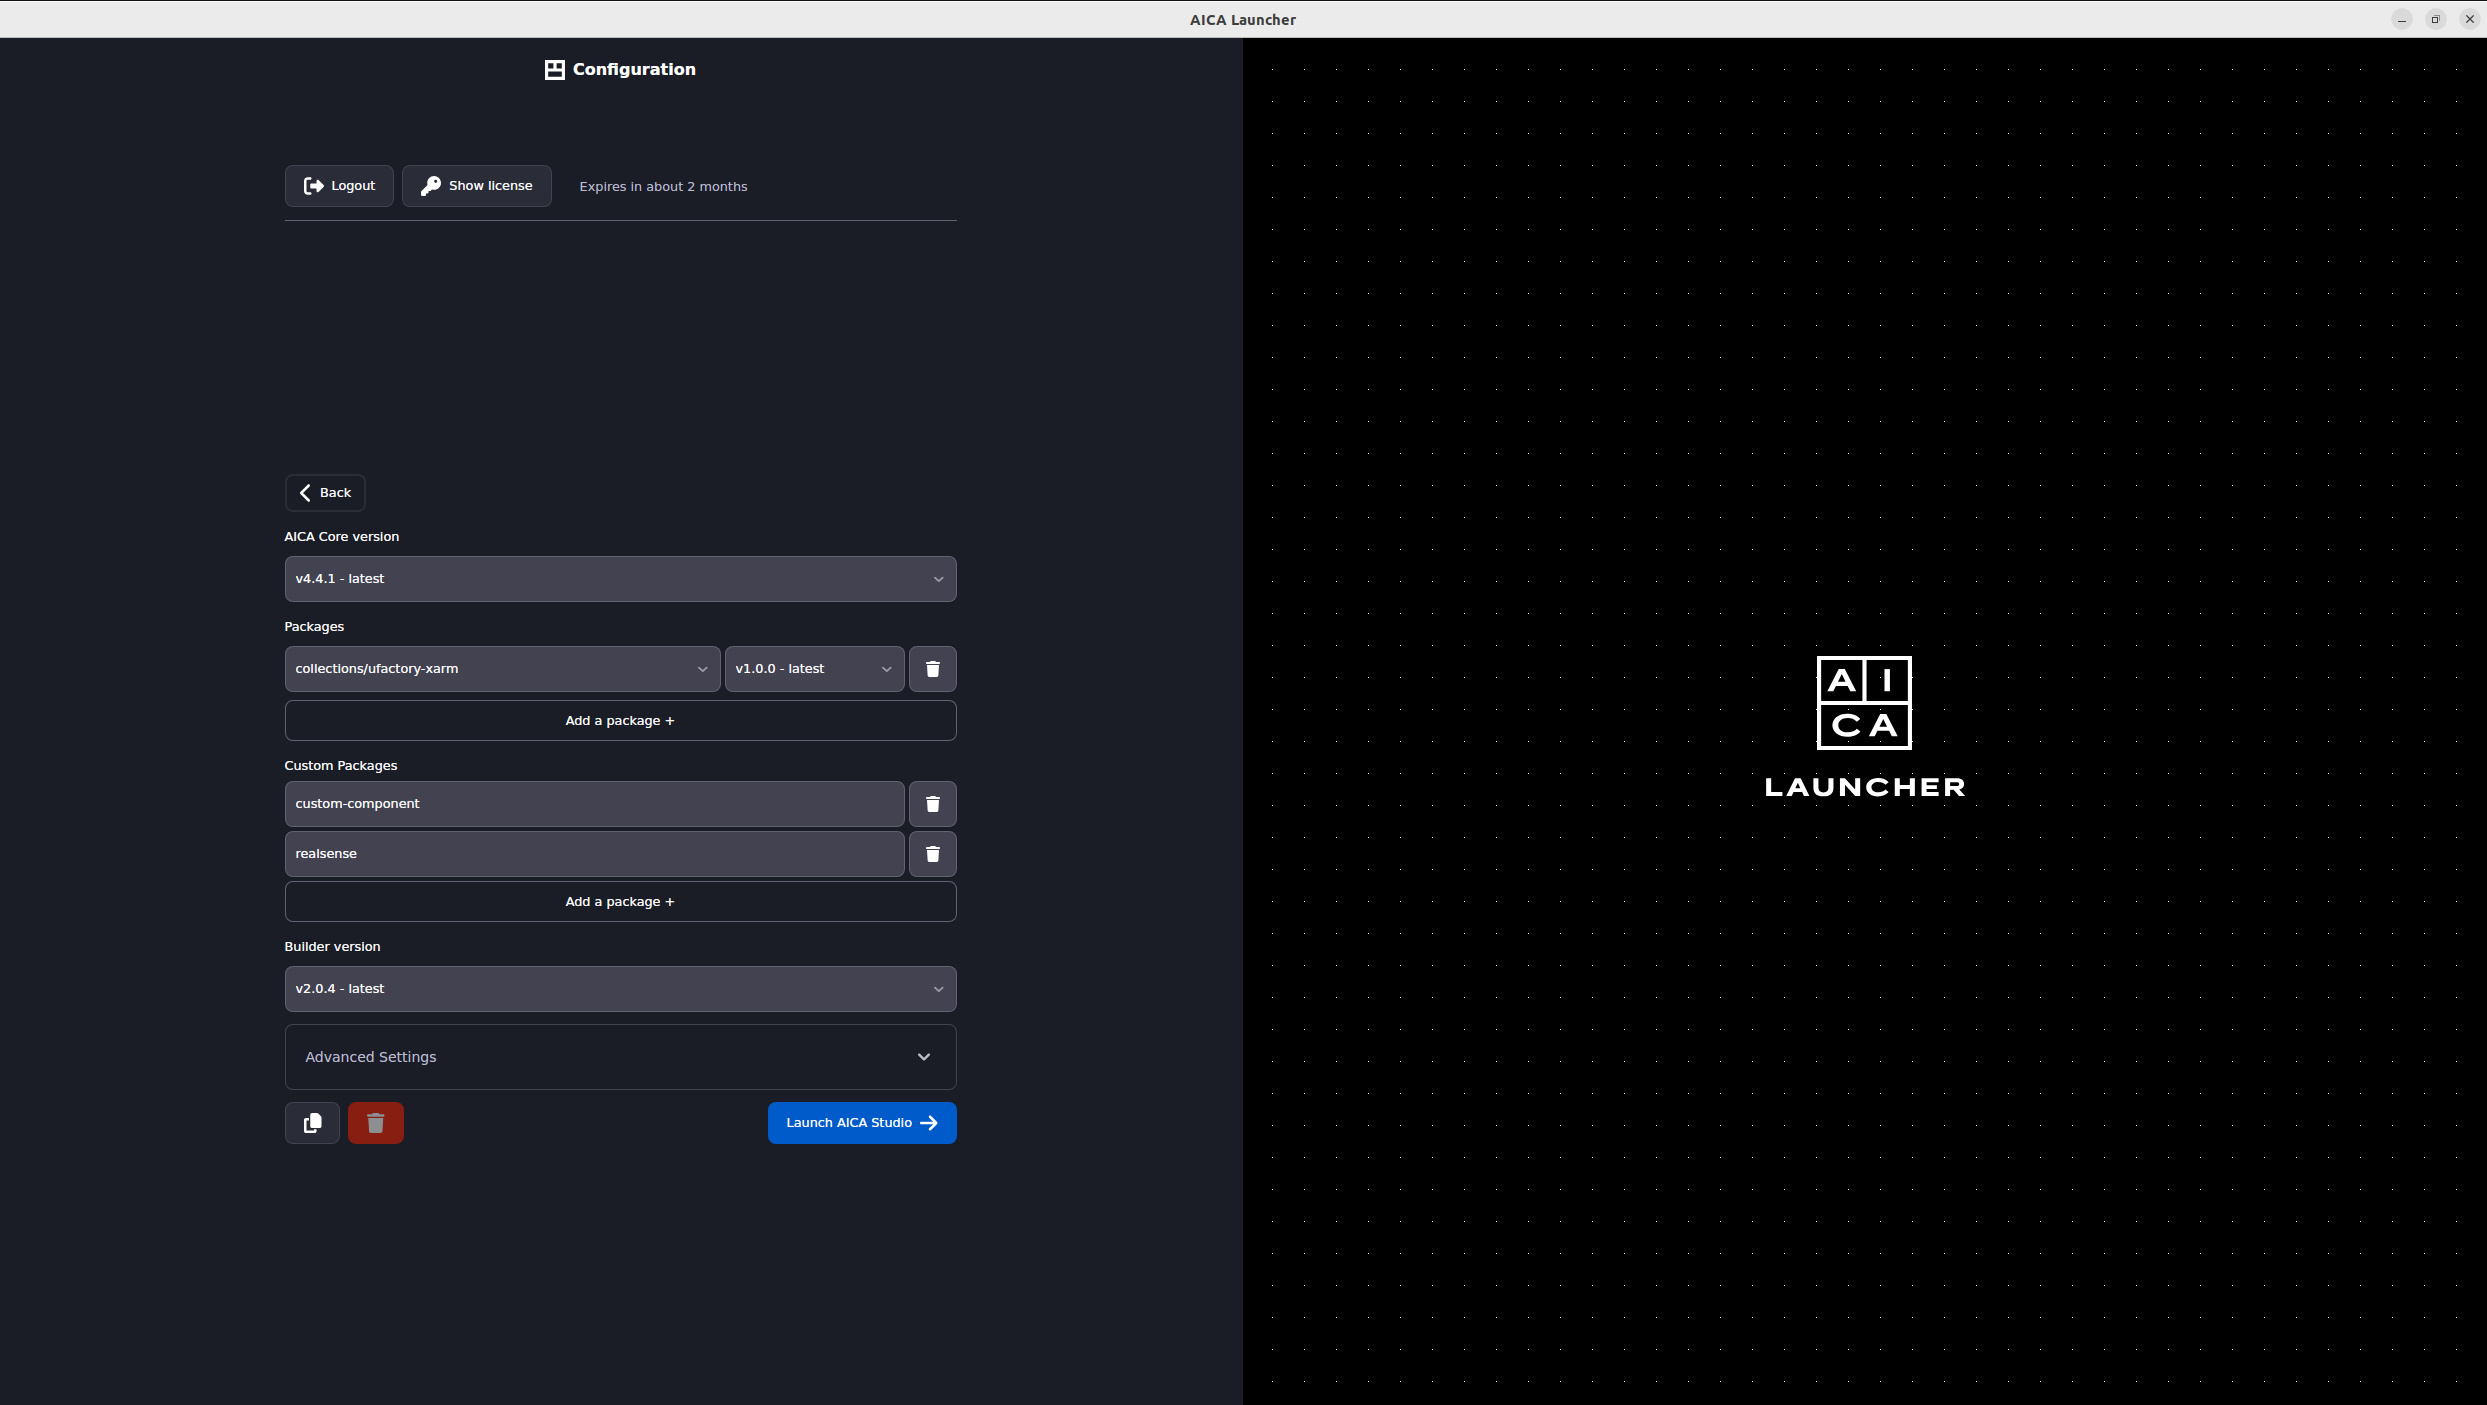
\includegraphics[width=0.8\textwidth]{assets/figures/AICA_Mainmenu.png}
    \caption{Page de démarrage de AICA Studio}
    \label{fig:aica_startup}
\end{figure}

\subsection{Interface de AICA Studio}
Le logiciel est relativement intuitif et facile à prendre en main pour ce qui est de la création de programmes et la connexion des blocs fonctionnels. Cependant à l'heure actuelle, il est nécesasire de comprendre et de maitriser des concepts de base de la programmation avec \gls{ros2} pour pouvoir comprendre et utiliser les différentes possibilités offertes par le logiciel. Il est donc recommandé de suivre les tutoriels et la documentation fournis par AICA ainsi que les ressources en ligne pour se familiariser avec les concepts de base de \gls{ros2} avant de se lancer dans la création de programmes.

Il est possible de créer des programmes de deux manières différentes avec AICA Studio :
\begin{itemize}
    \item En utilisant des blocs fonctionnels prédéfinis, qui permettent de créer des programmes de manière visuelle en connectant les blocs entre eux.
    \item En utilisant la fenêtre de programmation \gls{yaml}, qui permet d'avoir une vison plus detaillée du programme et de modifier les paramètres sans passer par la fenêtre de configuration des blocs.
\end{itemize}

\begin{figure}[H]
    \centering
    \begin{subfigure}{0.48\textwidth}
        \centering
        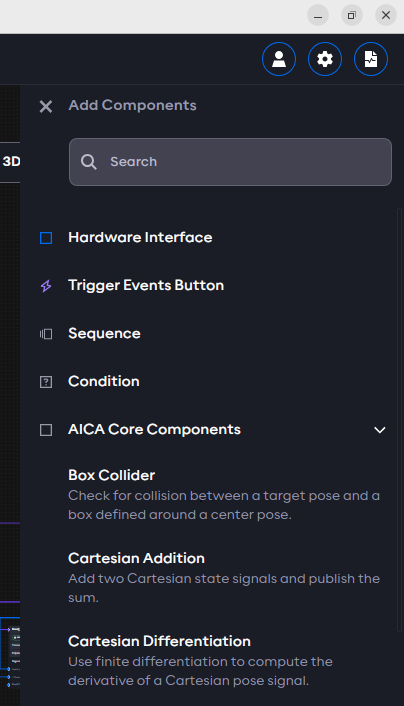
\includegraphics[width=0.95\linewidth]{assets/figures/AICA_blocs_fonct.png}
        \caption{Programmation par blocs visuels}
        \label{fig:prog_blocs_visuels}
    \end{subfigure}
    \hfill
    \begin{subfigure}{0.48\textwidth}
        \centering
        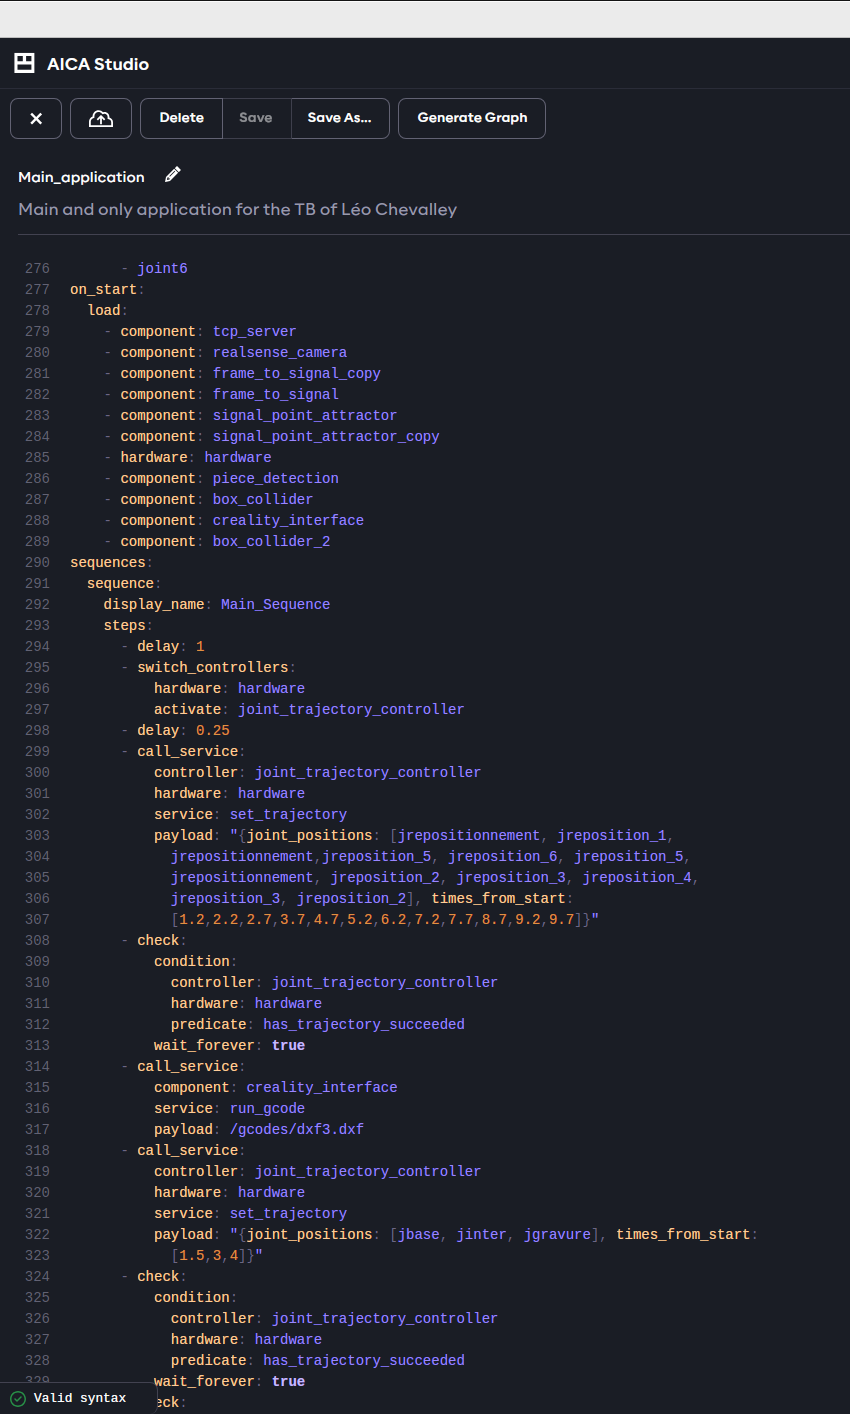
\includegraphics[width=0.95\linewidth]{assets/figures/AICA_Yaml.png}
        \caption{Programmation via YAML}
        \label{fig:prog_yaml}
    \end{subfigure}
    \caption{Comparaison entre la programmation visuelle et la programmation YAML dans AICA Studio.}
    \label{fig:comparaison_yaml_visuel}
\end{figure}

Concernant le reste de l'interface, le logiciel contient :

% Liste textuelle des éléments
\begin{itemize}
    \item Une barre de menu, qui permet d'accéder à la documentation, aux contrôles \gls{hardware} et à la page programmation par blocs (voir a).
    \item Un onglet réglages qui permet de redémarrer l'application, accéder au terminal et démarrer à \gls{rviz} (voir b).
    \item Un bouton pour accéder aux \gls{logs} de l'application (voir c).
    \item Des boutons d'actions pour le démarrage, l'arrêt et le rechargement du programme (voir d).
\end{itemize}

% Figure avec sous-figures légendées
\begin{figure}[H]
    \centering
    \begin{tabular}{cc}
        \begin{subfigure}{0.45\textwidth}
            \centering
            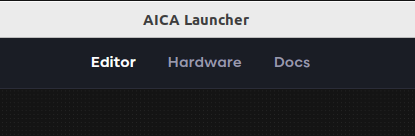
\includegraphics[width=0.9\linewidth]{assets/figures/AICA_barre_haute.png}
            \caption{Barre de menu}
            \label{fig:aica_barre_menu}
        \end{subfigure} &
        \begin{subfigure}{0.45\textwidth}
            \centering
            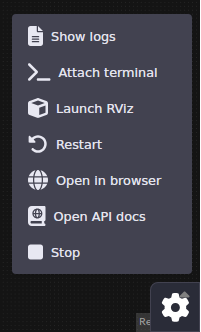
\includegraphics[width=0.9\linewidth]{assets/figures/AICA_rviz.png}
            \caption{Onglet réglages}
            \label{fig:aica_rviz}
        \end{subfigure} \\
        \addlinespace[0.5em]
        \begin{subfigure}{0.45\textwidth}
            \centering
            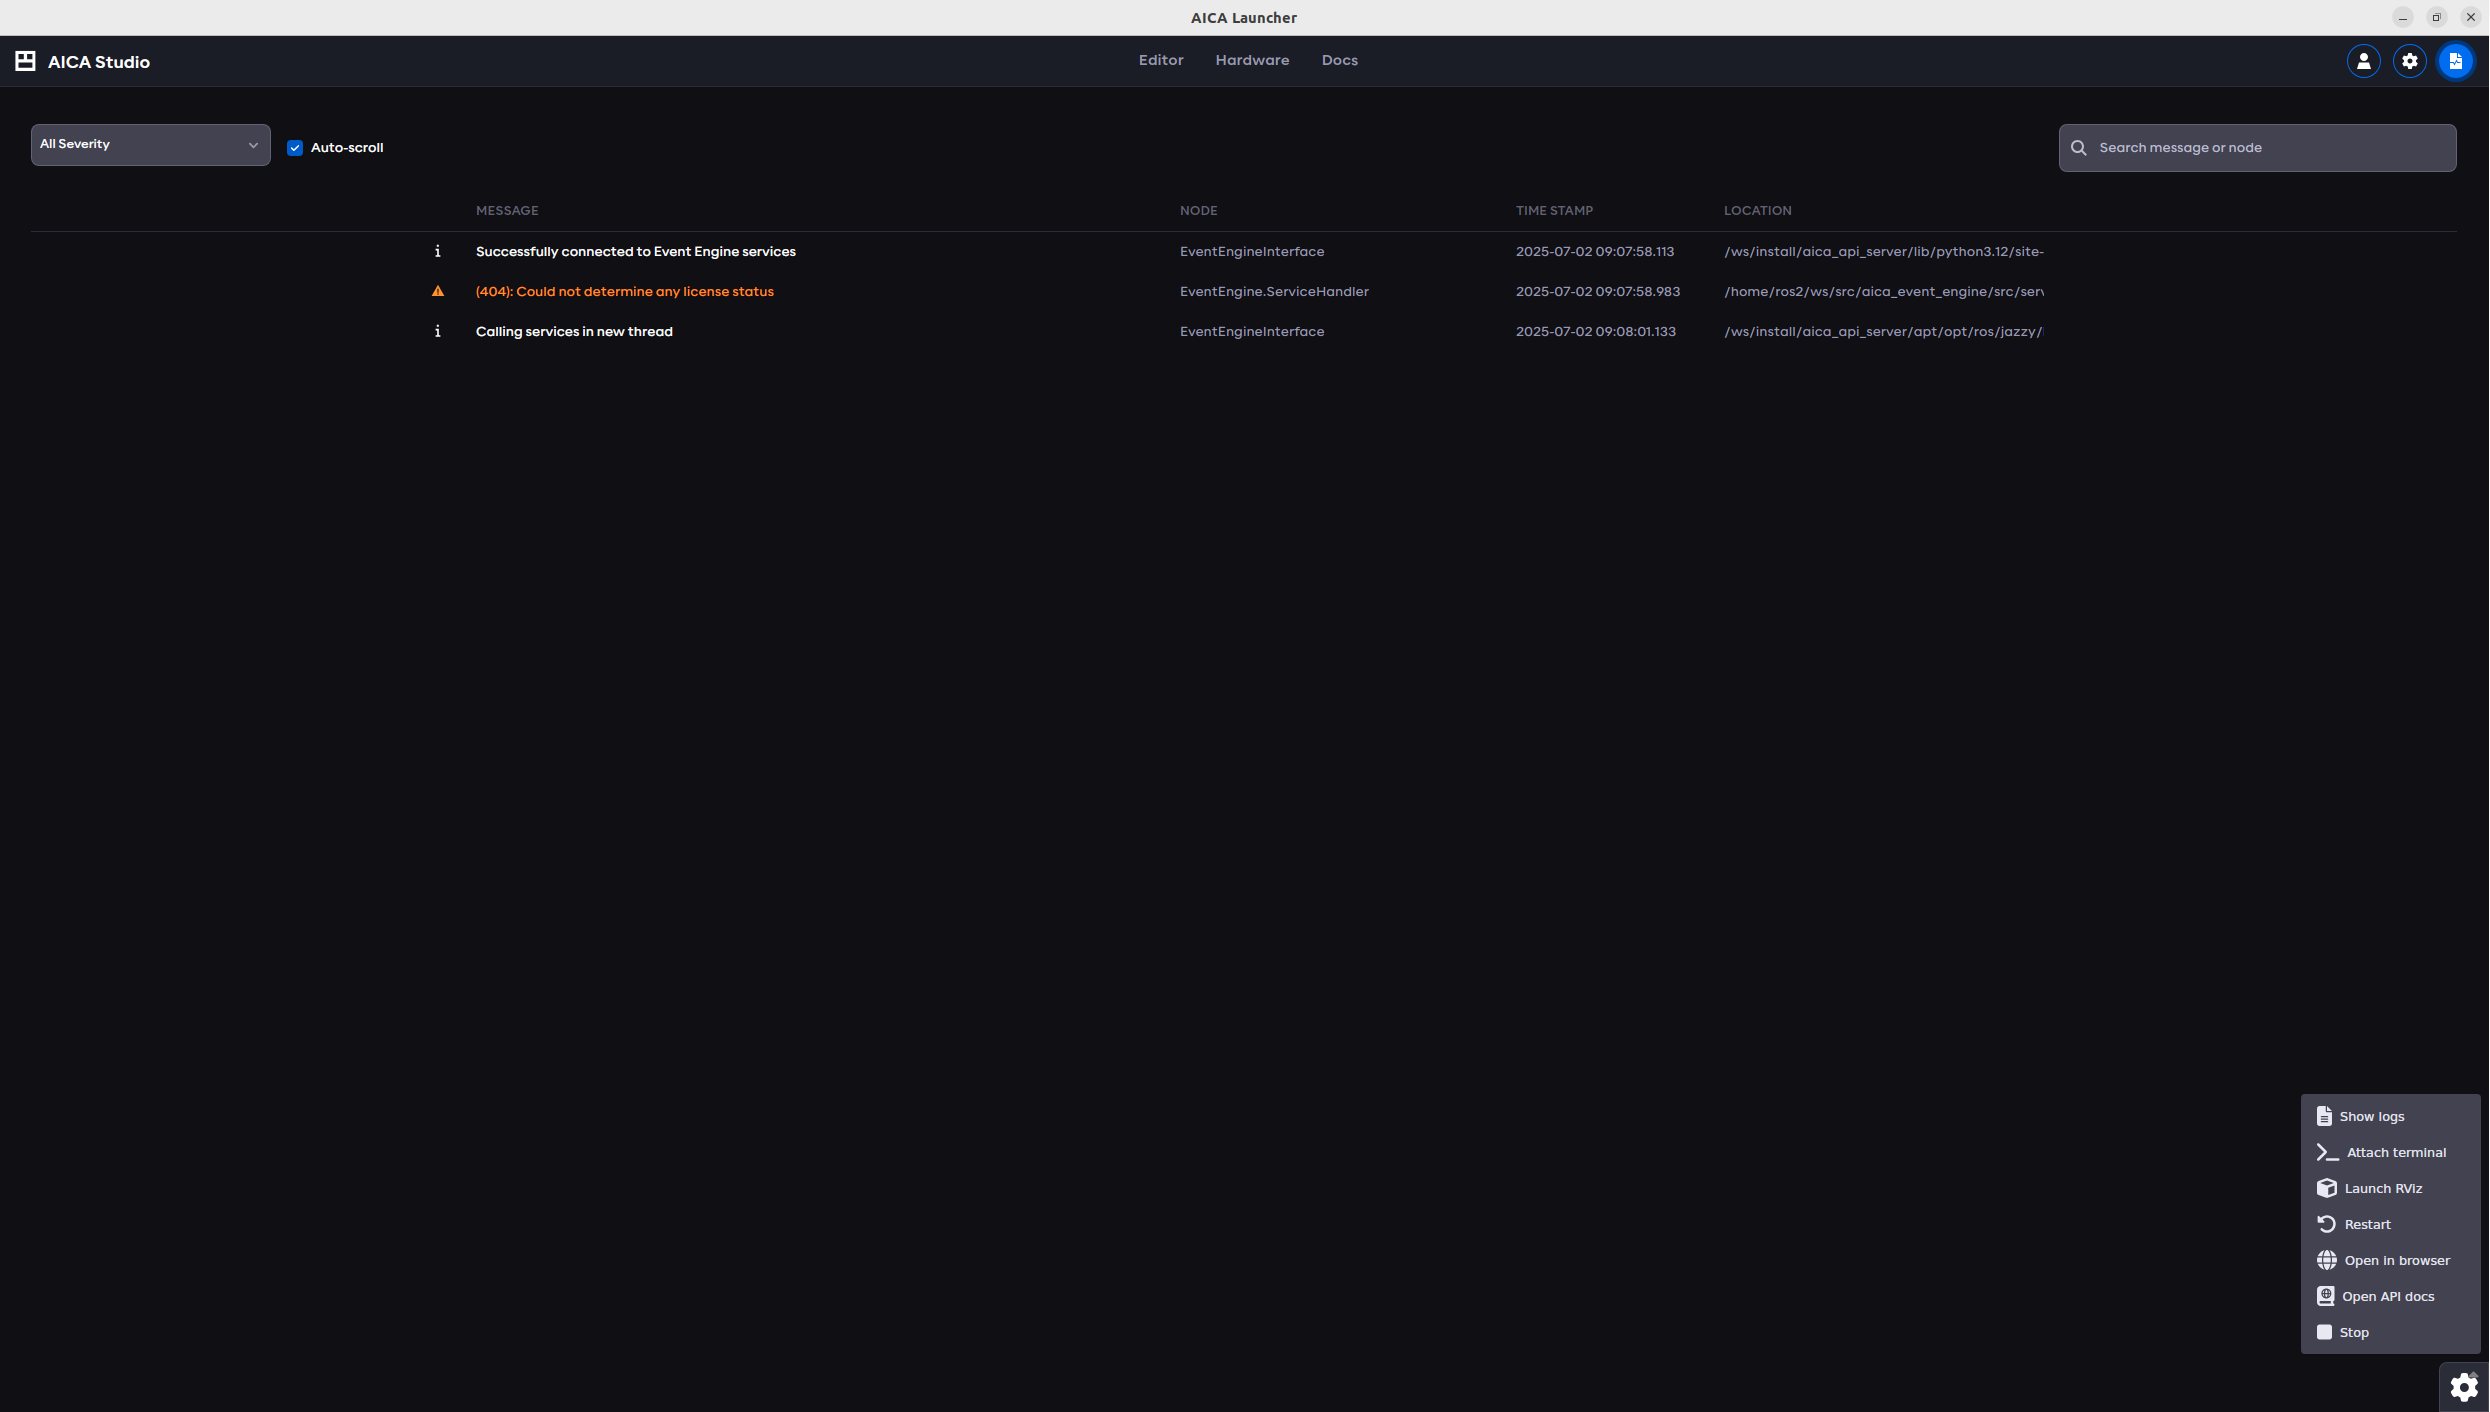
\includegraphics[width=0.9\linewidth]{assets/figures/AICA_logs.png}
            \caption{Bouton logs}
            \label{fig:aica_logs}
        \end{subfigure} &
        \begin{subfigure}{0.45\textwidth}
            \centering
            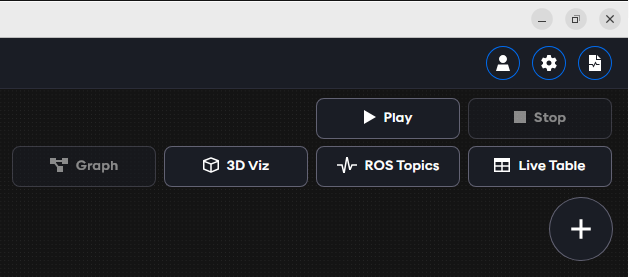
\includegraphics[width=0.9\linewidth]{assets/figures/AICA_play_pause.png}
            \caption{Boutons d'action}
            \label{fig:aica_play_pause}
        \end{subfigure}
    \end{tabular}
    \caption{Principaux éléments de l'interface de AICA Studio (présentation en grille 2x2).}
    \label{fig:aica_interface_elements}
\end{figure}

Ces éléments permettent de naviguer facilement dans l'application et d'accéder aux différentes fonctionnalités. L'interface est conçue pour être intuitive et facile à utiliser. malgré les limitations actuelles du logiciel et la nécessité de comprendre les concepts de base de \gls{ros2} ainsi que les premières versions de AICA Studio, l'interface utilisateur est à présent agréable à utiliser.

\section{Limites}
Bien que la station de gravure laser intelligente réponde aux besoins initiaux du projet, certaines limites ont été identifiées :
\begin{itemize}
    \item \textbf{Dépendance logicielle} : Le système repose sur des logiciels propriétaires (AICA Studio, UFACTORY) qui peuvent évoluer ou devenir obsolètes.
    \item \textbf{Sécurité publique} : Malgré les mesures prévues, la sécurité en contexte public dépend fortement de la vigilance de l'opérateur.
    \item \textbf{Flexibilité des scénarios} : Le système est optimisé pour la démonstration, mais moins adapté à une production industrielle ou à des pièces très variées.
\end{itemize}

Cette réflexion permet d'ouvrir le projet à de futures évolutions et d'envisager des applications plus larges ou plus exigeantes.



